\section{OpenFOAM}
\label{sec:OpenFOAM}

\subsection{Introduction}

OpenFOAM is an open source framework for computational fluid dynamics. It is entirely written in C++ and licensed under the GNU General Public License (GPL). OpenFOAM comes with basic meshing tools, various solvers and utilities to import meshes and export data for post processing. As opposed to many commercial packages the OpenFoam tools do not provide a graphical user interface. Instead the user has to edit configuration files within an OpenFOAM case and then run the solver in a UNIX-like fashion on the command line. One of the strengths of OpenFOAM is that custom solvers can be written or modified quickly because of its modular design and the usage of advanced C++ features.

\subsection{Mesh Representation}
\label{sec:meshRepresentation}

OpenFOAM supports unstructured polyhedral meshes with any number of faces. The mesh is described in the official Users Guide \cite{ug08} (chapter 5), the Programmers Guide \cite{pg08} (chapter 2.3) as well as in Jasak's PhD thesis \cite{jasak96} (chapter 3.2). Here I will recall a short summary. OpenFOAM stores the mesh in the following files\footnote{Located in \verb+constant/polyMesh+ in an OpenFoam case directory.}, which are generated by mesh utilities such as \verb+blockMesh+.

\begin{itemize}

	\item \verb+points+ Contains a list of coordinates of vertices. OpenFOAM implicitly indexes the points starting from 0 up to the number of points minus one.

	\item \verb+faces+ Contains a list of faces. The point indices defined in the \verb+points+ file are used to reference the vertices. It is distinguished between internal faces and boundary faces: Internal faces are between two cells and always have an owner and a neighbour cell assigned, while boundary faces lie on the boundary of the computational domain and just have an owner cell assigned (see below). Further a face normal is defined, so that it points outside of the owner cell. In case the face is a boundary face, the normal points outside of the computational domain.

The order of the vertices of a face is defined such that, if the normal vector points towards the viewer, the vertices are arranged in an anti-clockwise path. The faces are also implicitly indexed, starting with 0 for the first face.

It is common that the faces inside the simulation domain, called inner faces have a lower face label than those on the boundary, called boundary faces. OpenFOAM lets the user define various boundary conditions by referring a set of boundary faces.

	\item \verb+owner+ Each face is assigned an owner cell, in case of an internal face this is the cell with the lower label of the two cells adjacent to the face. The face normal can also be defined as pointing from the cell with the lower label to the cell with the higher label.

	\item \verb+neighbour+ Internal faces also have a neighbour cell. Since an internal face is always between two cells, the cell not being the owner is the neighbour cell. (Which is the cell with the higher label.) Faces lying on the boundary have no neighbour cell and are omitted in the neighbour list. Since some faces always lie on the boundary, this list has less items then the owner list.

	\item \verb+boundary+ The boundary file contains a list of patches which refer to a set of boundary faces.
	
\end{itemize}

\subsection{The Lagrangian Framework}
\label{sec:lagrangianFramework}

OpenFOAM includes a Lagrangian framework which was originally developed to simulate Diesel droplets \cite{nordin00}. The simplest Lagrangian library allows the simulation of solid particles which are moved by the Eulerian field. The work carried out here is based on the \verb+solidPartilce+ library.

\begin{figure}[H]
  \centering
  \includegraphics[scale=0.6]{content/gfx/solidParticleClasses.pdf}
  \caption{Class diagram outlining the solidParticle library.}
  \label{gfx:solidParticleClasses}
\end{figure}

Figure \ref{gfx:solidParticleClasses} shows the most important classes belonging to the solidParticle library. Note that, for the sake of simplicity not all class members are shown. The particles are stored in a doubly linked list. The particle tracking algorithm is implemented in a flexible way: The most basic functionality is in the \verb+Particle+ class via the \verb+trackToFace()+ function. Functionality specific to a certain particle type, such as the drag model, is implemented in the \verb+solidParticle+ class. The \verb+solidParticle+ class provides the \verb+move()+ method which is called from the \verb+solidParticleCloud+ class for every particle. Using the specific drag model the destination for a particle is estimated, \verb+trackToFace()+ is then called with the before calculated destination.

\paragraph{Usage of curiously recurring template patterns}

When looking at the classes of the \verb+solidParticle+ library a remarkable circular dependency between derived classes can be found. For example the classes \verb+Particle+ and \verb+solidParticle+ in the Lagrangian framework. \verb+solidParticle+ is derived from the \verb+Particle+ class template which takes the type of the derived class as template argument.

\begin{figure}[H]
  \centering
  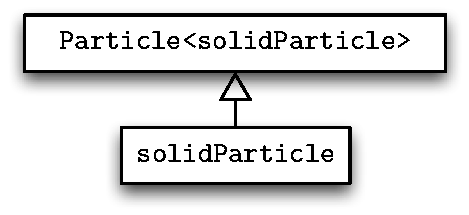
\includegraphics[scale=0.6]{content/gfx/solidParticle.pdf}
  \caption{Illustration of circular dependencies in OpenFOAM using templates and inheritance.}
  \label{gfx:solidParticle}
\end{figure}

% TODO Why exactly is this allowed? By the standard templates are instantiated 
% first and then?

The dependency goes in one direction via inheritance and in the other direction via templates. This pattern was named ''Curiously Recurring Template Pattern (CRTP)'' by James Coplien in 1995 \cite{coplien95}. It can be used to implement static polymorphism without the need to use virtual functions, as illustrated in the example below.

\begin{lstlisting}
#include <cstdio>

template <class DerivedType>
struct A {

    void doSomething() {
        static_cast<DerivedType&>(*this).doSomethingElse();
    }
};

struct B: public A<B> {

    void doSomethingElse() {
        
        printf("Hello from B!\n");
    }
};

struct C: public A<C> {
    
    void doSomethingElse() {
        
        printf("Hello from C!\n");
    }
};


int main() {
    
    B b;
    b.doSomething();
    C c;
    c.doSomething();
    
    return 0;
}

// Output

Hello from B!
Hello from C!

\end{lstlisting}

As mentioned before this idiom is used in the Lagrangian classes\footnote{This can be found in the OpenFOAM source tree in the directory \verb+src/lagrangian+}. The \verb+Particle+ class is declared as follows:

\begin{lstlisting}
template<class ParticleType>
class Particle : public IDLList<ParticleType>::link {
    //..
};
\end{lstlisting}

And the \verb+solidParticle+ class as follows:

\begin{lstlisting}
class solidParticle : public Particle<solidParticle> {
    //..
};
\end{lstlisting}

The particle class can now call members which are to be defined in their derived classes using a static cast on the \verb+this+-pointer.

\begin{lstlisting}
static_cast<ParticleType&>(*this)
\end{lstlisting}

Using a reference to the derived type it can be checked weather the particle is of a special type as done on line 299 from the file \verb+Particle.C+:

\begin{lstlisting}
//..
else if (static_cast<ParticleType&>(*this).softImpact())
{

//..
\end{lstlisting}

This is just one example in which this idiom is used and there are many more within the code of OpenFOAM.

\subsection{Parallelization and Support for GPUs}

The OpenFOAM code is mostly sequential C++ code. Larger simulations can be decomposed into various domains and multiple instances of a solver can be launched which communicate using the message passing interface (MPI) \cite{openfoamParallel}. While OpenFOAM currently does not support fine grained parallelism, it has recently been shown that OpenFOAM could benefit a hybrid parallelization model where OpenMP is used in addition to MPI for the fine grained parallelization on each host \cite{liu11}.

There is officially no support for GPU computing in OpenFOAM, however various third-party solutions exist. The \cite{speedit} SpeedIT tools make it possible to use OpenFOAM with CUBLAS, Nvidia's implementation of BLAS (Basic Linear Algebra Subprograms). OFGPU \cite{ofgpu} runs the Preconditioned conjugate gradient solver for symmetric matrices (PCG) and the Preconditioned biconjugate gradient solver for asymmetric matrices (PBiCG) on the GPU by using the CUSP \cite{cusp} library, a library for sparse linear algebra and graph computations on the GPU.